\section{Introduction}

Image-based modeling and simulation is becoming an increasingly important analytic and predictive tool for a variety of medical and engineering applications. Some examples include patient-specific diagnosis and treatment \cite{neal2010current}, large-scale \textit{in silico} trials \cite{viceconti2016silico}, medical device design, computer-assisted surgery, and, in the industrial realm, analysis of as-built structures and components \cite{bradley2005advances}. Image-based modeling and simulation comprises a long chain of methodological elements, which can be organized into several major task domains:
\begin{enumerate}
\item
segmentation of the raw image, 
\item
creation of a boundary representation (b-rep) of the problem domain,
\item
generation of a suitable volume mesh (finite elements or other), 
\item
assignment
of boundary conditions and constitutive models, 
\item
the physics-based
simulation itself on the volume mesh, and
\item
visualization and interrogation of the simulation results.
\end{enumerate}
This article focuses on the second of these task domains:  creation of a b-rep given a segmented image (i.e. an image mask).  
The b-rep creation step itself typically consists of several sub-steps.  
We describe our approach alongside three alternatives, and offer both quantitative and visual comparisons.

We use the term {\em b-rep} instead of {\em surface}
in order to emphasize certain properties that are essential to the target
application:  namely, the b-rep must be closed and oriented (and therefore
``watertight''), and manifold in the case of only a single material domain, as is our present focus.  We further stipulate that the b-rep should consist of an assemblage of simple polygonal facets defined by shared vertices and 
edges.  I.e., we desire explicit geometry and topology, and not an implicit definition based, say, on level surfaces. In addition, the b-rep facet size should be controllable as a matter of input, in view of the fact that the volume mesh (e.g. finite elements) is typically much coarser than the voxel grid.

We preview our approach to the segmented-image-to-b-rep step in Figure \ref{}, which outlines, in flowchart form, the steps in our proposed workflow alongside those of three alternatives.  The names of the alternative workflows are for identification purposes only; they generally reflect a key component of the respective workflow.  However, it bears emphasis that all four processes consist of unique workflows with multiple interdependent steps. They each have their advantages, characteristics, and weaknesses, which are products not only of the performance of the individual methodological elements of each workflow, but also of their interplay.  Our main interest here is in the overall performance of our workflow next to the three comparators, which we try to assess both quantitatively and visually in section \ref{}.  The four workflows will be explained in greater detail in section \ref{}.

\begin{figure}[t]
	\centering
		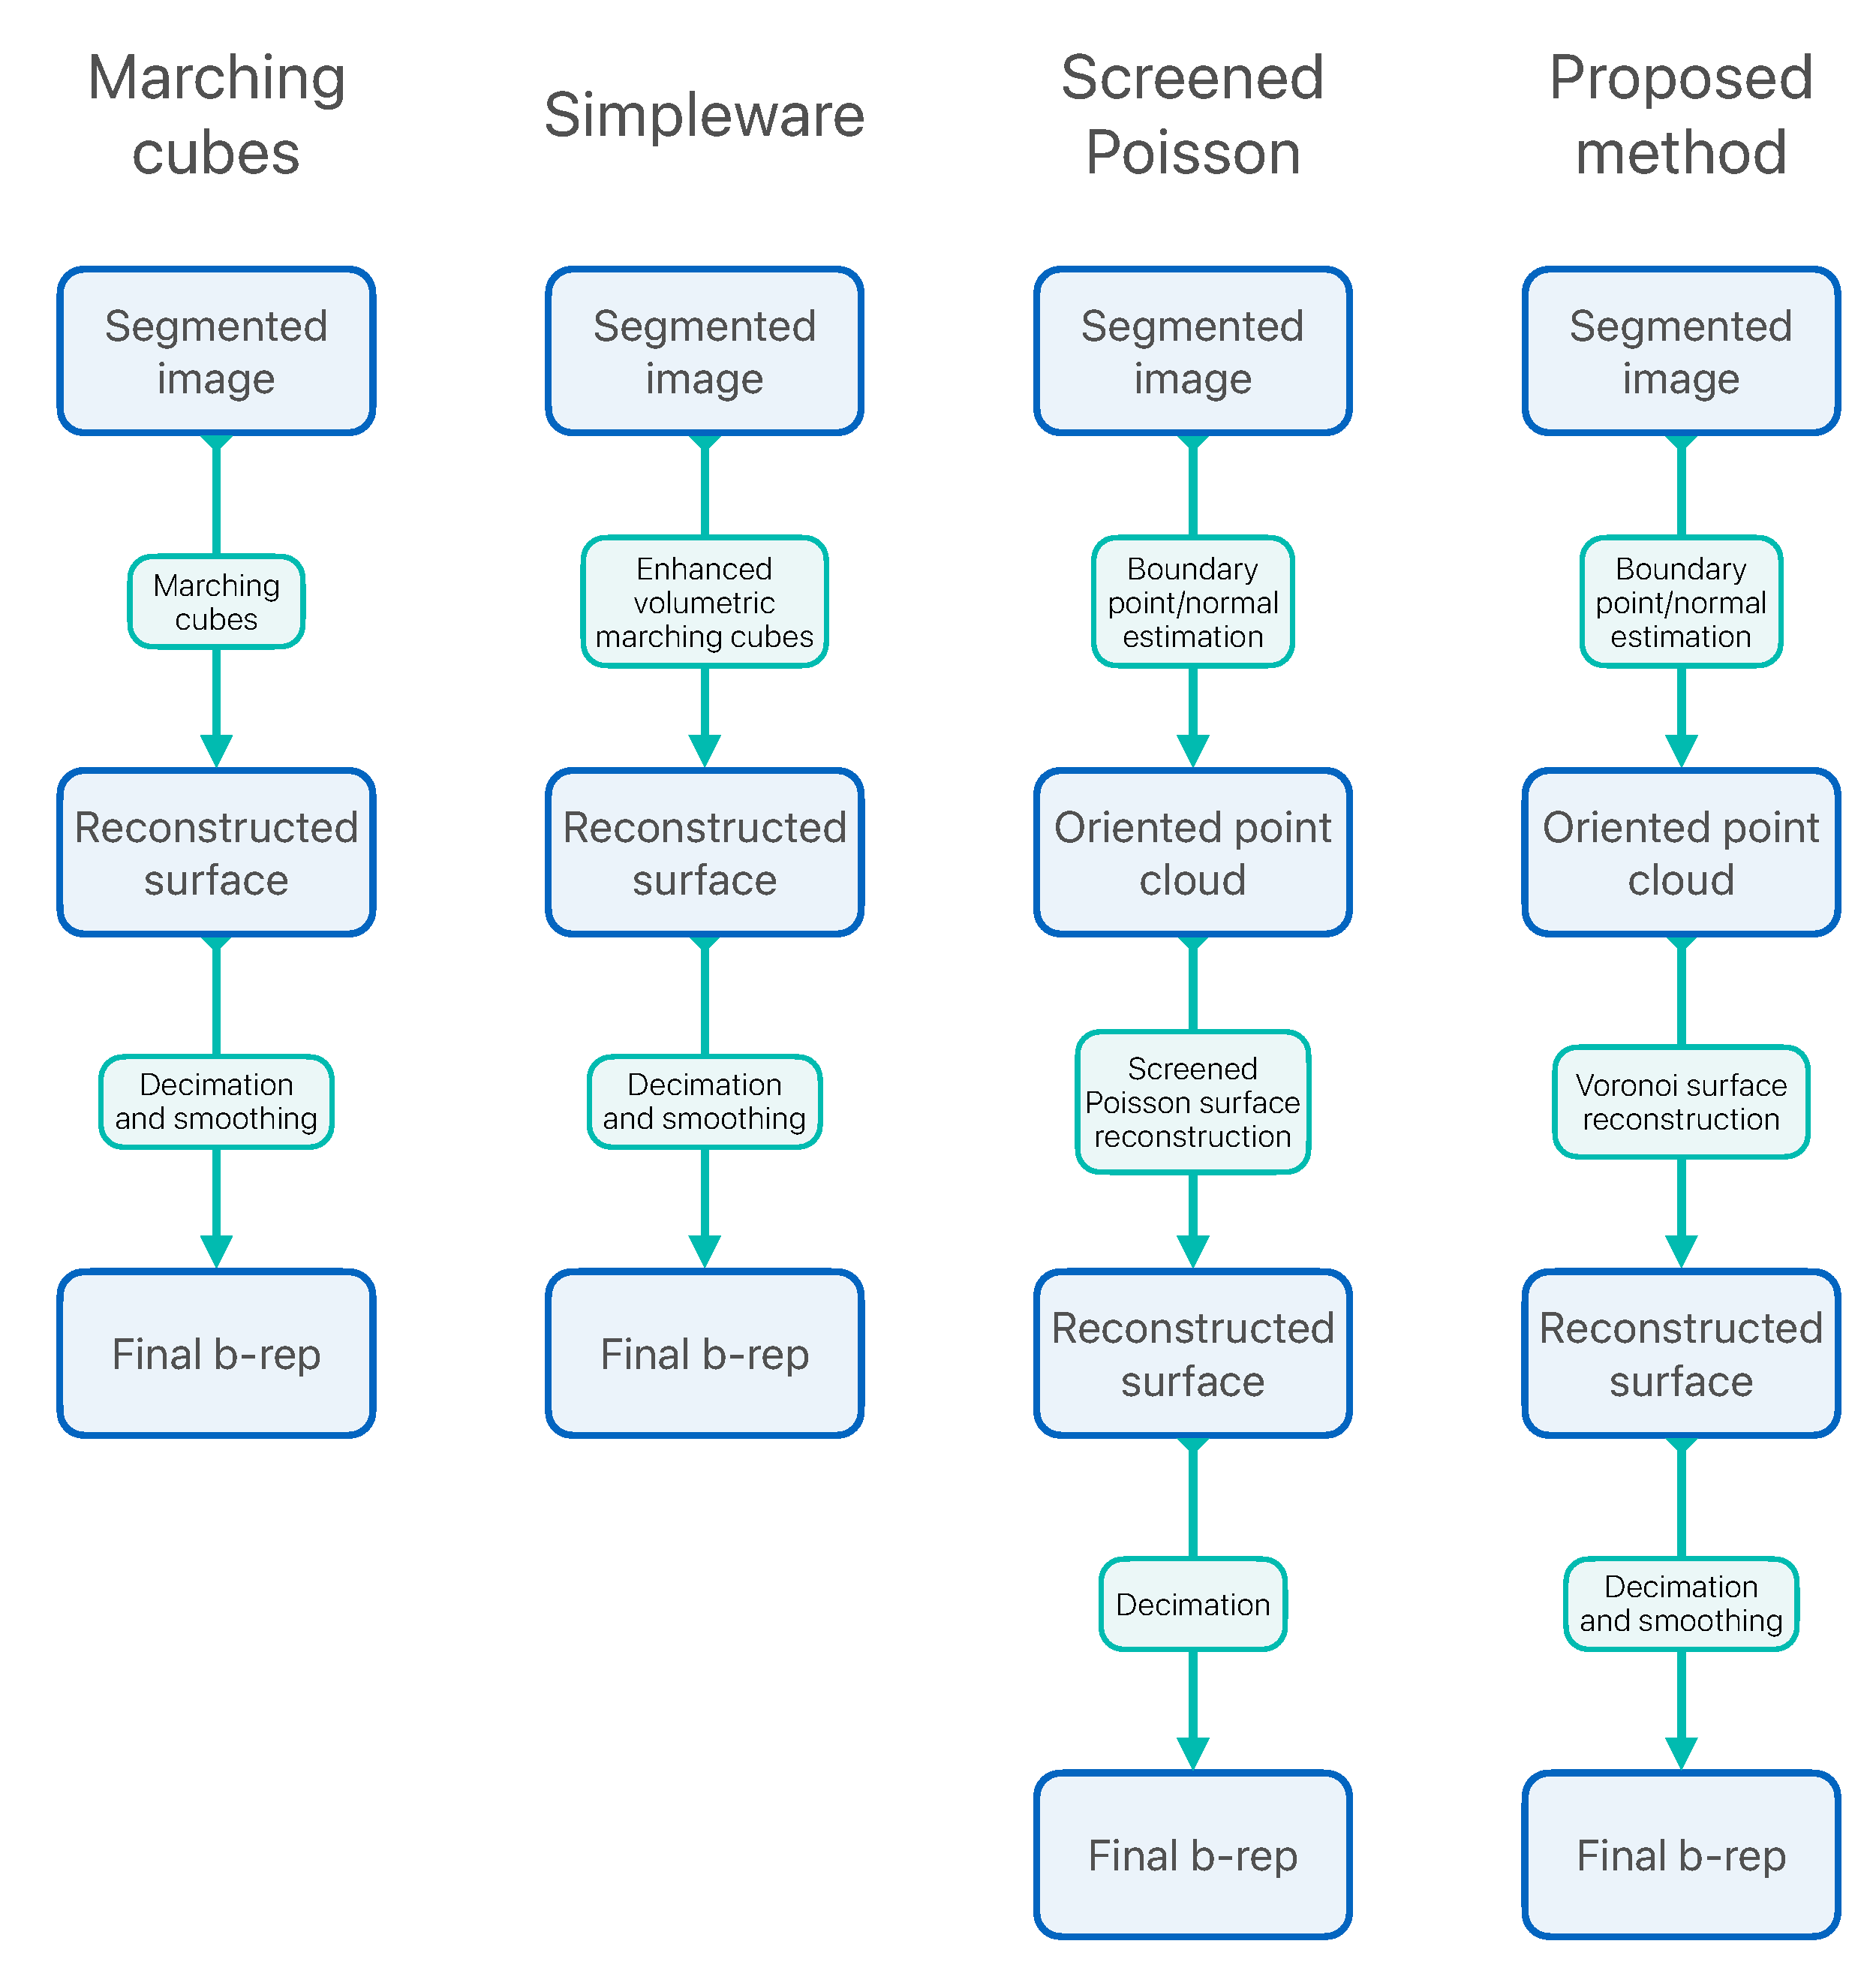
\includegraphics[scale=0.3]{media/flowchartNew.pdf}
	\caption{Flowcharts of different techniques to generate b-reps from image masks.}
	\label{fig:flowchart}
\end{figure}\noindent

A main objective of this work is to
contribute to a high degree of automation in the overall image-to-analysis process.  We therefore place particular emphasis on 
computational {\em robustness}:  given a segmented image that is in some sense noisy, our goal is that the b-rep should nevertheless ultimately support the generation of a computable volume mesh.  In rough terms, if the image mask is good enough to define a sensible problem domain, the resulting b-rep should reliably exhibit suitable water-tightness and topological-correctness properties.

In most practical circumstances, the final volumetric mesh
must be much less dense than the voxel grid.  This fact, together with the assumed presence of noise in the image mask, means that the image-to-b-rep step must engender an element of smoothing in its functioning.  Such smoothing inevitably requires an algorithm with heuristic features.  ``Noise,'' in the context of a discrete image mask, really means pollution in the form of miscolored voxels.  These can (and often do) occur as isolated red voxels surrounded by black voxels near the ``legitimate'' surface.  Of course, any arbitrary coloring of a voxel grid defines a valid b-rep consisting of red-black surfels, but this ``literal'' b-rep generally consists of jagged surface features and many small isolated islands and holes.  The job of the image-to-b-rep algorithm, then, is to produce a geometry that is suitable in scale for the subsequent volumetric-meshing step, while smoothing out the fine-scale pollution present in the image mask, but not unduly rounding any legitimate sharp features.  Clearly there is a measure of subjectivity in this task:  noise and sharp features are not always distinguishable using objective means.
